\chapter{Productivity tools}
As we we began the development of the Easy Web Content Site Builder from scratch, it gave us the opportunity to set-up a bunch of productivity tools. These tools are about automatize tasks, enhance code quality, debug, teamwork, documentation.

None of the following tools were implemented before I arrived in Hindsite Interactive. 
\section{Pear}

PEAR is a framework and distribution system for reusable PHP components. It allows to easily install, remove and update PHP libraries and packages by using simple command line.

\lstset{language=bash}
\begin{lstlisting}[label=pear-install,caption=Installation of pear packages]
C:\...>pear channel-discover channelname
C:\...>pear install --alldeps channelname/packagename
\end{lstlisting}

\section{Phing}

To work more efficiently, we implemented automatic build task tools . Phing is a build tool written in PHP. It is very similar to the famous ANT. Phing build tasks have been set to automatize js/css minification with the YUI Compress tool.
Right now we can use it to automate deployment and development.
\begin{itemize}
\item automatic js / css minify for release
\item automatic backup
\item automatic database deployment
\item generate php documentaion from comments
\end{itemize}

Phing uses pear to be installed automatically.

\lstset{language=bash}
\begin{lstlisting}[label=phing-install,caption=Installation of Phing]
C:\...>pear channel-discover channelname
C:\...>pear install --alldeps channelname/packagename
\end{lstlisting}

The build is configured with an xml file : build.xml. It allows to program automated tasks called targets. Targets can be combined and ordered.
Obfuscate JavaScript or CSS file would have been a very repetitive and boring task to do manually. This tool allows to keep the code non obfuscated for development environment (easy to debug and read), and obfuscated in production environment (lighter, faster and harder to read).

\lstset{language=Ant}
\begin{lstlisting}[label=phing-build,caption=Example of Phing build.xml]
<project name="EasyWebSite" basedir="." default="info">
	<property name="ProjectVersion" value="0.0.1" />
	<target name="minify-js">
		<minify targetDir="${releaseDirectory}/Framework/public/js/"
				yuiPath="${buildScriptsDirectory}/yuicompressor-2.4.2.jar">
			<fileset dir="${applicationDirectory}/Framework/public/js/">
			<include name="**/*.js"/>
			<exclude name="library/**"/>
			</fileset>
		</minify>
	</target>	
	<target name="zip-backup"
		description="Creates a backup of the project">
		<echo msg="Backup to zip archive"/>
		<copy file="build.xml" tofile="build.xml.backup" overwrite="true"/>
		<mkdir dir="${backupDirectory}" />				
		<zip destfile="${backupDirectory}/ews_backup-${ProjectDate}.zip">
		<fileset dir=".">
			<include name="build.xml" />
			<exclude name="build/**"/>
			<exclude name="docs/**"/>
			<include name="src/**" />			
		</fileset>
		</zip>
	</target>
	<target name="build-all" depends="cleanup , setup-environments, prepare-libs , execute-phpdoc, execute-jsdoc , deploying-debug, deploying-release, minify-js ,minify-css, deploy-database"
		description="deploys full environment">       
		<echo msg="Fin du build" />		
	</target>		
</project>
\end{lstlisting}

\section{Subversion}

Subversion is a version control system. It allows to keep track on modifications of files revision after revision. A system like this is very important to use in a team environment. For several reasons.

\paragraph*{Critic portions of code}
When working on important pieces of code the developer is often afraid to introduce bugs or to make the application crash. With a version control system, he can roll-back to previous stable versions of the code easily. So he can experiment new features with more confidence. 

\paragraph*{Debug}
If a bug is introduced, the developer can check what were the modifications in which files by using a 'diff' tool to compare two revisions of a the same file.

\begin{figure}[!ht]
\centering
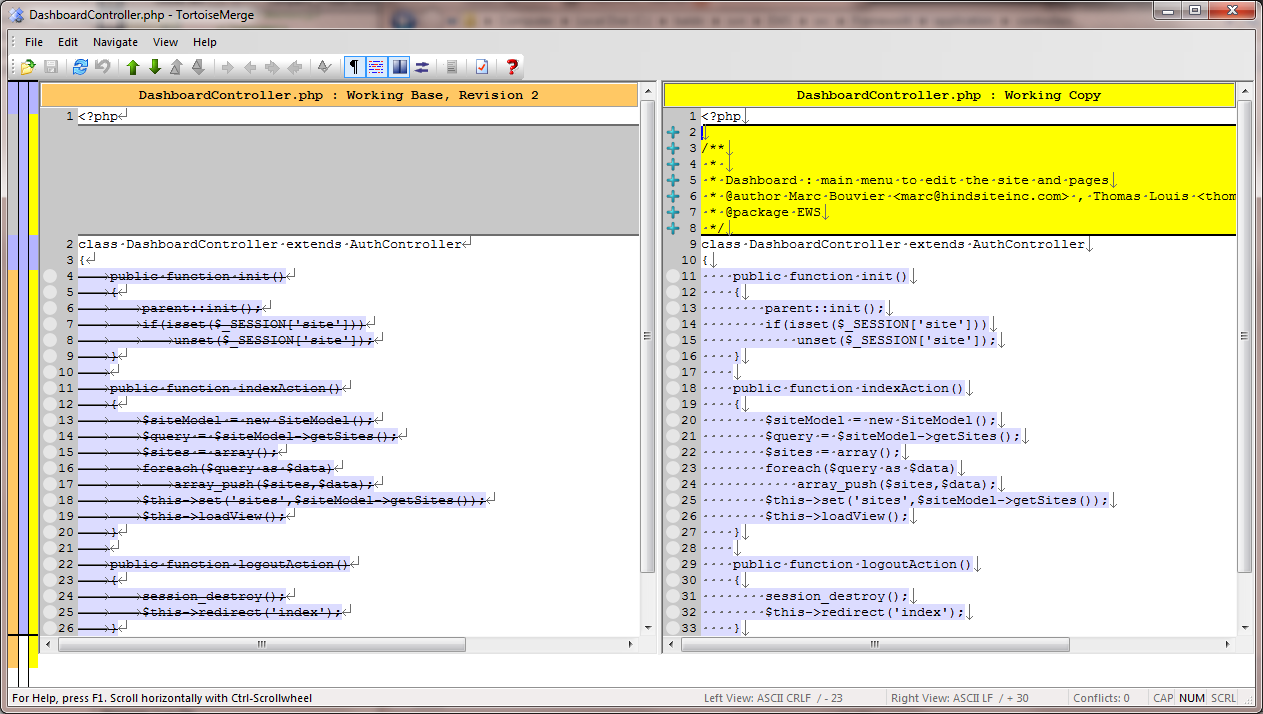
\includegraphics[width=.85\textwidth]{img/diff.png}
\caption{Diff tool}
\label{figure:diff}
\end{figure}

\paragraph*{Team-work}
When working in on a project with several developers, it is very important to work on the same versions of the project's file. Subversion stores the project in a repository from where the developers download incrementally the latest modifications of the files. So, only new or modified files are updated. Two developers may work on the same file at the same time because Subversion possess file merge and conflict resolution capabilities. It avoids overwriting a file that another developer would have modified.

\section{Code documentation}
Our applications and precisely the Site Builder project need to be maintenable and scalable. 

When I arrived at Hindsite Interactive and began working on the Easy Web Content project, I had to read a lot of documentation about the architecture of different components, but there was no document of the actual functions in the code. To understand the code and be able to debug it, having code documentation is a must.
\subsection{PHPDoc}
PhpDoc is a PHP framework that allows to generate web documentation of a project by using comments in the PHP code.

\begin{figure}[!ht]
\centering
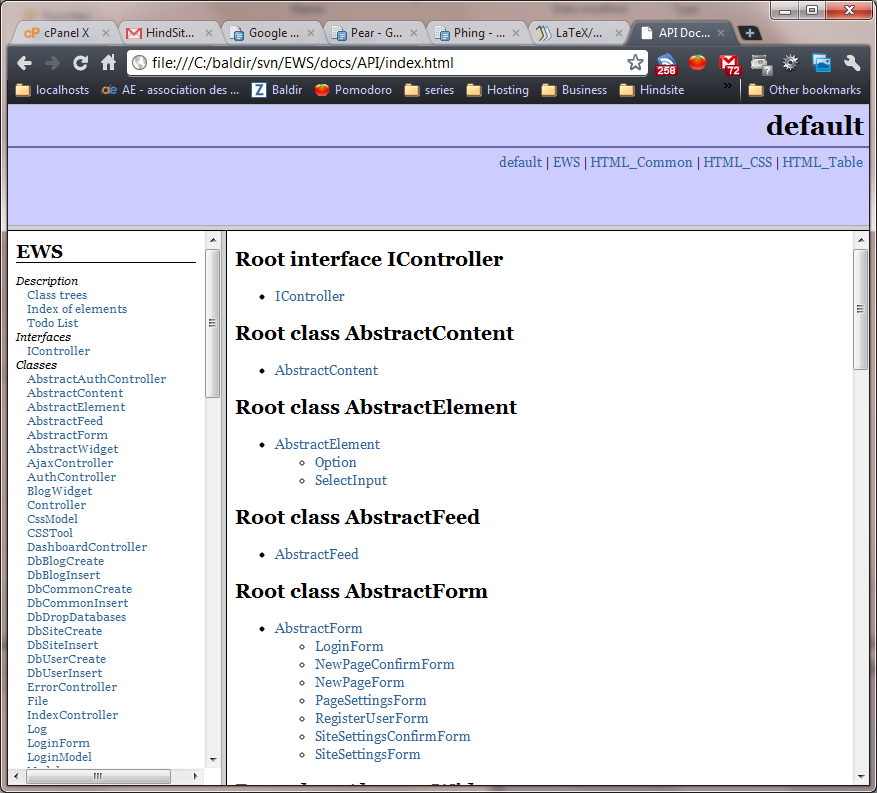
\includegraphics[width=.55\textwidth]{img/phpdoc.png}
\caption{Generated PHP Documentation from PHP code}
\label{figure:phpdoc-web}
\end{figure}

\lstset{language=PHP}
\begin{lstlisting}[label=phpdoc-code,caption=PHP documentation in a PHP class]

/**
 * 
 * Controller. 
 * The controller receives input and initiates a response by making calls on model objects.
 * A controller accepts input from the user and instructs the model and viewport to perform
 * actions based on that input.
 * @author Marc Bouvier <marc@hindsiteinc.com> , Thomas Louis <thomas@hindsiteinc.com>
 * @package	EWS
 */
class Controller implements IController{
	
	/**
	*	Boolean remains to false if no error occured, else set to true
	*	@var boolean
	*/
	protected static $error = false;

	/**
	 * 
	 * Constructor for the class Controller
	 * @param unknown_type $controllerName
	 * @param unknown_type $action
	 */
	public function __construct($controllerName, $action, $queryString=array()) 		{
		//some code
	}
\end{lstlisting}


\subsection{JSDoc}
JsDoc is a Javascript framework that allows to generate web documentation of a project by using comments in the Javascript code.

\begin{figure}[!ht]
\centering
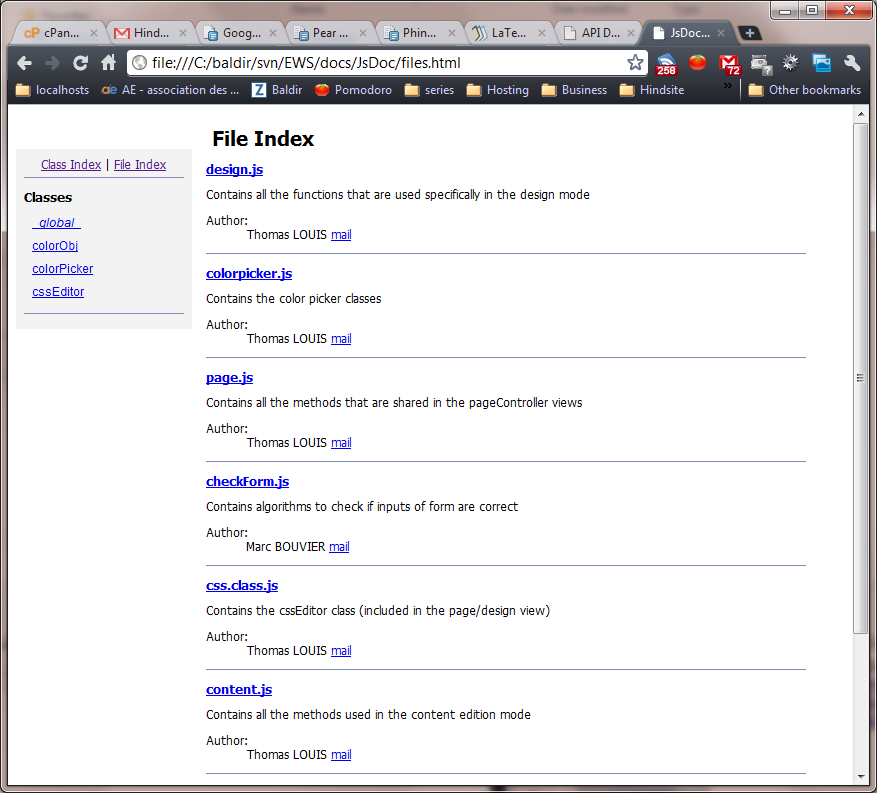
\includegraphics[width=.55\textwidth]{img/jsdoc.png}
\caption{Generated Javascript Documentation from Javascript code}
\label{figure:jsdoc-web}
\end{figure}

\lstset{language=Javascript}
\begin{lstlisting}[label=jsdoc-code,caption=Javascript documentation in a Javascript class]
/**
*	@fileOverview Contains the cssEditor class (included in the page/design view)
*	@author Thomas LOUIS <a href="mailto:thomas@hindsiteinc.com">mail</a>
*/

/**
*	@class Base class to set the css string and elements that the user wants to modify
*	@author Thomas LOUIS <a href="mailto:thomas@hindsiteinc.com">mail</a>
*/
cssEditor = function(target)
{
	/**
	*	Target of the click (it is a jQuery Object)
	*	@type Object
	*/
	this.target = target;

/**
*	Sets the inline property so that the user can see right away the changes applied to his page
*	@param {String} cssProperty The css property to be applied
*	@param {String} cssValue The property value
*	@todo Look and change the function
*/
cssEditor.prototype.setCss = function(cssProperty,cssValue)
{
	// some code		
}

\end{lstlisting}

\section{Netbeans}

Since we used Object Oriented Programming with PHP we had more needs of tools 
to write the code. Especially an IDE \footnote{Integrated Development Environment}.

\begin{itemize}
\item code autocompletion
\item code navigation
\item code syntax recognition
\item classes heritage detection
\end{itemize}


\section{Mantis}
Hindsite Interactive uses a lot Google documents to track tasks and issues. This allows to work on the same documents with other people of the team. The problem of this system is that it is not very efficient to manage tasks and bugs. It is like you track bugs in a Word document.

We have set up a bug tracker for internal use called Mantis it allows fast bug reporting. It allows Prioritization, importance management ... and assignment of issues to resolve. This allows everyone to keep track of the specific tasks they need to accomplish, and the bugs they need to resolve.


\begin{figure}[!ht]
\centering
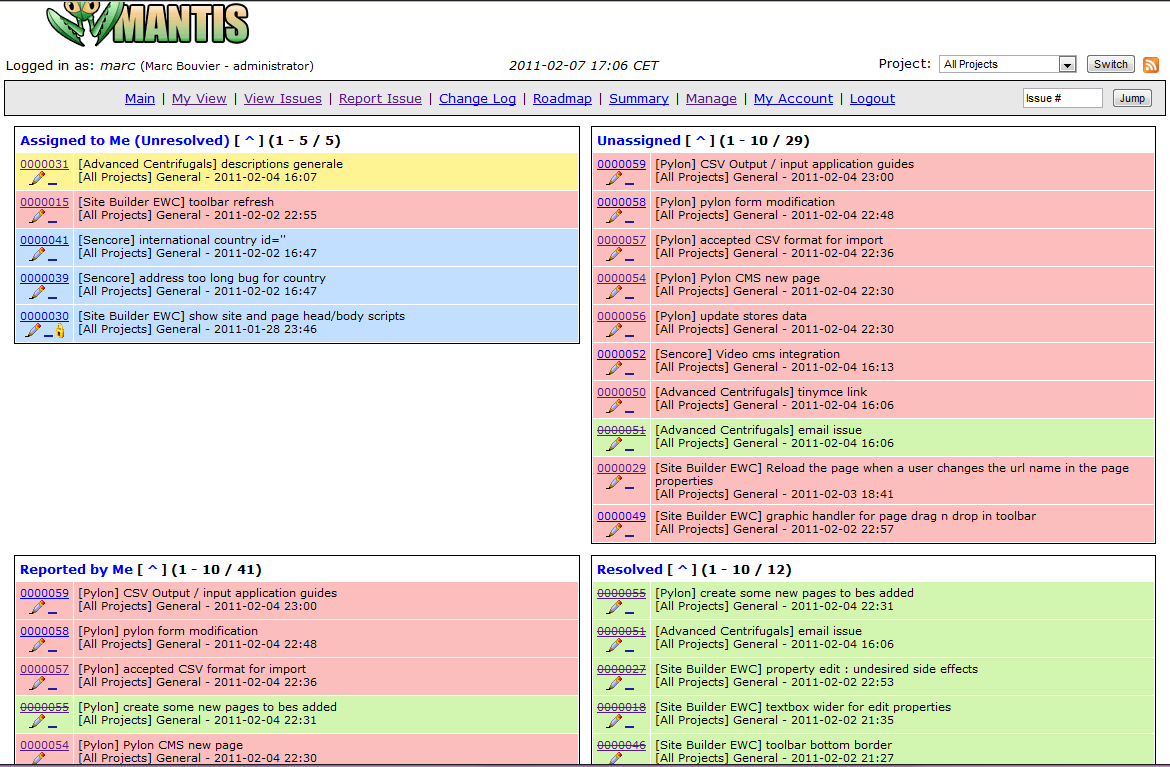
\includegraphics[width=.85\textwidth]{img/mantis.png}
\caption{Mantis tasks and issues multi-project view}
\label{figure:mantis}
\end{figure}
 

